\documentclass[preprint,11pt]{elsarticle}
\usepackage[T1]{fontenc}
\usepackage[a4paper,margin=25mm]{geometry}
\usepackage{amsmath,amssymb,booktabs,tabularx,graphicx}
\usepackage{lineno}
\usepackage{xurl}
\usepackage[hidelinks]{hyperref}
\usepackage{listings}
\usepackage{placeins}
\lstset{basicstyle=\small\ttfamily,breaklines=true,columns=fullflexible,frame=single}
\journal{SoftwareX}
\linespread{1.05}
\setlength{\emergencystretch}{2em}
\makeatletter
\def\ps@pprintTitle{\let\@oddhead\@empty\let\@evenhead\@empty
  \def\@oddfoot{\footnotesize\itshape Draft for SoftwareX\hfill 21 October 2026}
  \let\@evenfoot\@oddfoot}
\makeatother
\begin{document}
\begin{frontmatter}
\title{LaplaceX: fitting exponential mixtures with wavelet rate proposals}
\author[itmo]{Artem Vozmishchev\corref{cor}}
\ead{a.vozmishchev@niuitmo.ru}
\cortext[cor]{Corresponding author.}
\affiliation[itmo]{organization={ITMO University},city={Saint Petersburg},country={Russia}}
\begin{abstract}
A small reconstruction residual can conceal an incorrect number of exponential
components. LaplaceX estimates component counts, rates, and amplitudes through
wavelet proposals followed by joint nonlinear fitting. We evaluate its logarithmic
time representation using compiled linear-coordinate and rate-grid controls that
share the optimizer and model-selection code. On a separated three-mode fixture,
logarithmic coordinates reduce elapsed time by factors of 7.22 and 9.99 against
these controls; the linear-coordinate detector is faster on a close pair.
The wavelet route recovers 480/480 counts on reused validation and regression
mixtures, compared with 479/480 for variable projection. A new noise and
rate-separation sweep exposes a harder limit: correct counts fall to 708/960,
versus 737/960 for variable projection. Local information bounds and true-count
fits distinguish favorable estimation conditions from weak identifiability.
Measured fluorescence tails demonstrate the interface and reveal sensitivity
to tail selection. The principal benefit is reduced search cost for decays
with separated time scales; component counts, parameter errors, and
reconstruction quality must still be assessed separately.
\end{abstract}
\begin{keyword}
exponential fitting \sep wavelets \sep logarithmic time \sep model selection \sep Laplace transform \sep scientific Python
\end{keyword}
\end{frontmatter}
\linenumbers

\section*{Code metadata}
\begingroup\small
\noindent\begin{tabularx}{\textwidth}{@{}>{\raggedright\arraybackslash}p{0.28\textwidth}>{\raggedright\arraybackslash}X@{}}
\toprule
Current code version & 1.0.0\\
Permanent link to code used & \url{https://github.com/BRUTALLOLOL/LaplaceX/tree/ff164d309a89b72eaafb2c58eb83430399ba9b24}\\
Code versioning system & Git\\
Legal code license & MIT\\
Software languages and tools & Python, C++17, pybind11, CMake, scikit-build-core\\
Operating environments and dependencies & Python 3.10 or later; NumPy 1.24 or later; a C++17 compiler for source builds. Wheels are built for Linux, Windows, and macOS.\\
Distribution & \url{https://pypi.org/project/LaplaceX/1.0.0/}\\
Documentation & \url{https://github.com/BRUTALLOLOL/LaplaceX/blob/ff164d309a89b72eaafb2c58eb83430399ba9b24/README.md}\\
Support & \url{https://github.com/BRUTALLOLOL/LaplaceX/issues}; \href{mailto:a.vozmishchev@niuitmo.ru}{a.vozmishchev@niuitmo.ru}\\
\bottomrule
\end{tabularx}
\endgroup

\section{Motivation and significance}
Exponential mixtures describe decay and relaxation measurements, but an accurate
reconstruction need not identify their physical components. Nearby rates can
compensate for one another, while weak components contribute little residual
energy. Identifiability therefore matters alongside optimization speed
\cite{istratov}.

Logarithmic-time derivatives have long been used to approximate relaxation
spectra, including the Alfrey and Schwarzl--Staverman approaches
\cite{alfrey,schwarzl}. Automatic component estimation also predates this work:
Provencher's Fourier method supplied counts and initial parameters
\cite{provencher}. Other established routes include Prony methods
\cite{prony}, Hankel subspace methods \cite{hsvd}, and matrix pencils
\cite{pencil}. Variable projection eliminates linear amplitudes from nonlinear
optimization \cite{golub}; projected fitting can reduce costs for large datasets
\cite{hokanson}. NNLS \cite{nnls} and CONTIN \cite{contin,continprogram}
address constrained or regularized distributions, whose discretization and
regularization differ from selecting a small finite mixture.

LaplaceX integrates multiscale rate proposals, joint fitting, and practical
count selection in a Python library. Its contribution is a reusable
implementation and a controlled evaluation of search cost. The logarithmic
transformation is an established representation, and no logarithmic
computational-complexity claim is made. We examine both its advantages and
conditions where a specialist comparator performs better.

\section{Software description}
\subsection{Interface and scope}
A C++17 extension performs the numerical work; Python functions accept NumPy
arrays and return an \texttt{ExponentialComponents} container. Users can inspect
rates, amplitudes, and decay times, reconstruct signals, and export results.
Decomposition fits real decaying exponentials with signed amplitudes and can
recognize constant-only signals. It does not estimate oscillation frequencies.
The tests below use positive mixtures. Relative absolute-amplitude weights,
called \texttt{significances} in version 1.0.0, are descriptive weights rather
than statistical probabilities.

The package also provides adaptive Gauss--Kronrod forward quadrature, spline
integration for sampled inputs, and Weeks--Laguerre inversion \cite{weeks}.
These are separate routines. This article focuses on exponential decomposition;
it attributes no wavelet gain to the forward or Weeks algorithms.

\subsection{Logarithmic-time proposals and joint refinement}
For observations
\begin{equation}
y_i=\sum_{k=1}^{K}A_k\exp(-\lambda_k t_i)+\varepsilon_i,
\qquad \lambda_k>0,
\label{eq:model}
\end{equation}
let $x=\log t$. A single component has the derivative profile
\begin{equation}
-\frac{d}{dx}f(e^x)=A h(x+\log\lambda),
\qquad h(z)=\exp(z-\exp z).
\label{eq:profile}
\end{equation}
Its peak occurs at $x=-\log\lambda$, with height $A/e$. Rate changes translate
one profile, making a common scale range useful across decades
(Figure~\ref{fig:log}). Overlap and observation-window truncation still limit
resolution.

\begin{figure}[htbp]
\centering
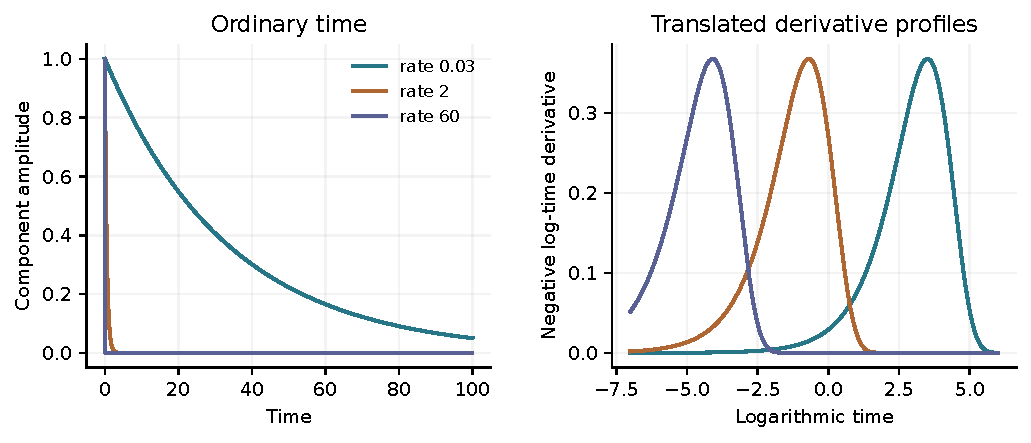
\includegraphics[width=.92\textwidth]{figures/log_time_profiles.pdf}
\caption{Equal-amplitude analytic components at rates 0.03, 2, and 60. Ordinary
time compresses fast decays near the origin; differentiation with respect to
logarithmic time produces translated profiles. This illustrates the coordinate
representation, without implying an identifiability guarantee.}
\label{fig:log}
\end{figure}

Defaults use 256 interpolation points uniform in $x$ and sixteen Mexican-Hat
scales on 0.05--0.5 log-time units, bounded below by 1.25 grid spacings.
Constant extension and discrete constant cancellation limit boundary artifacts.
Gaussian-derivative zero crossings are established multiscale features
\cite{marr}. Here, branches linked from fine to coarse scales initialize
several rates together; branches that later merge remain candidates.
A scale-dependent localization correction supplies approximate starting rates.

Scaled Householder QR initializes amplitudes. An analytic-Jacobian
Levenberg--Marquardt iteration then refines amplitudes and logarithmic rates
jointly on the original observations, reusing QR reductions across damping
trials. This native solver uses joint optimization; the specialist comparator
below uses variable projection. Interpolation affects proposals, not the
precision grid of the final fit.

Residual searches condition proposed components against current amplitude and
rate directions. For independent sample noise, interpolation $P$ and derivative
filtering $H$ give
\begin{equation}
\operatorname{Var}[(HP\varepsilon)_j]
=\sigma^2\sum_i(HP)_{ji}^2.
\label{eq:noise}
\end{equation}
Weights are accumulated per original observation, accounting for reuse during
interpolation. Cached filter norms reduce repeated work. This calculation does
not provide a multiple-testing guarantee for linked crossings.

BIC \cite{schwarz}, refitted deletions, conditional amplitude screening, and
boundary checks select a count within a user-specified budget. Automatically
estimated noise may be recalibrated from residual MAD near the noise level.
These are heuristic safeguards. The public API can additionally retry a
rate-grid search; that retry is disabled in the primary evaluation.

\section{Examples and evaluation}
\subsection{One configuration for the primary results}
The primary configuration is the log-wavelet route with default detector
settings, at most five components, and \texttt{auto\_deflate=False}.
The same configuration is used for synthetic recovery, matched native timing,
and the experimental example. Public-default retry is reported separately.
For example:
\begin{lstlisting}[language=Python]
import numpy as np
from laplacex import decompose

t = np.geomspace(0.002, 400.0, 600)
y = np.exp(-t[:, None] * [0.03, 2.0, 60.0]) @ [0.7, 1.3, 0.5]
fit = decompose(t, y, auto_deflate=False)
print(np.sort(fit.rates))
y_fit = fit.reconstruct(t)
\end{lstlisting}
This clean example returns rates 0.03, 2, and 60, with maximum reconstruction
error $4.44\times10^{-16}$ using the installed release.

\subsection{Comparators and the coordinate control}
The external native harness compiles an unchanged copy of the released core
and a coordinate-control copy. Both use the same compiler, wrapper, QR/LM
solver, noise rules, selection code, and component budget. The control samples
an affine function of ordinary time over the same coordinate span, with the
same 256 points and relative filter widths. It locates extrema of
$-t(G_b*f)'(t)$ using first and second Gaussian derivatives and converts peak
time to reciprocal rate. Thus both detectors target the same physical
quantity. The comparison changes finite-grid allocation and smoothing geometry
together; it does not establish an advantage over every linear-time detector.
A native 64-rate grid supplies a third matched control.

The specialist comparator uses exact variable-projection residual derivatives,
signed linear amplitudes, positive bounded rates, and two deterministic starts
for each count one through five. BIC selects the count. It is implemented with
SciPy \cite{scipy}; its timing includes Python callbacks. The matrix-pencil
comparator uses a truncated-SVD Hankel pencil followed by variable-projection
refinement and BIC selection. It is evaluated only on originally uniform
samples, without interpolating logarithmic samples. These are documented
implementations, not exhaustive searches over specialist methods or settings.

\subsection{Matched timing and rate proposals}
Twelve existing 600-sample fixtures include separated and close rates,
1000:1 amplitude cases without noise, and three Gaussian-noise realizations.
All fixtures were exposed during development, including those historically
named holdouts. Seven shuffled repetitions follow one warmup, with one BLAS
thread. Setup, input/output conversion, and fitting are timed; imports and
reference generation are excluded.

Measurements use an Intel Core i7-7700HQ, nominal 2.80 GHz, Windows x64,
Python 3.14.7, NumPy 2.5.3, SciPy 1.18.1, and Zig 0.16.0/Clang 21.1.0 with
C++17 and \texttt{-O3}. The Balanced power plan is recorded; clocks and thermal
conditions are not fixed. Table~\ref{tab:research-timing} and
Figure~\ref{fig:matched} retain every fixture and fixed comparator.

\begin{table}[htbp]
\centering\small
\caption{Median milliseconds from seven shuffled repetitions after warmup. Log, linear, and grid routes use the same compiled optimizer and wrapper; variable projection uses SciPy callbacks. All fixtures are development-exposed. $\dagger$ marks a route that fails the count/accuracy target in at least one repetition; its time is still reported.}\label{tab:research-timing}
\begin{tabular}{@{}lrrrr@{}}
\toprule
Fixture & Log & Linear & Grid & VarPro \\
\midrule
Single & 0.15 & 0.19 & 0.16 & 8.17 \\
Two uniform & 2.89 & 2.97 & 4.40 & 26.22 \\
Wide three A & 1.36 & 21.00 & 30.39 & 274.51 \\
Wide two & 0.83 & 2.41 & 4.30 & 22.05 \\
Wide three B & 1.23 & 8.88 & 12.29 & 64.59 \\
Close pair & 7.96 & 6.80 & 9.78 & 36.82 \\
Weak fast & 2.11 & 194.04 & 11.20 & 81.57 \\
Weak middle & 1.95 & 7.46 & 9.77 & 48.92 \\
Weak slow & 1.99 & 7.41 & 10.11 & 64.84 \\
Noise 7 & 2.66 & 5.76 & 13.69 & 236.88 \\
Noise 19 & 2.19 & 4.52 & 11.98 & 146.06 \\
Noise 41 & 2.15 & 5.82 & 13.48 & 488.80 \\
\bottomrule
\end{tabular}
\end{table}


\begin{figure}[htbp]
\centering
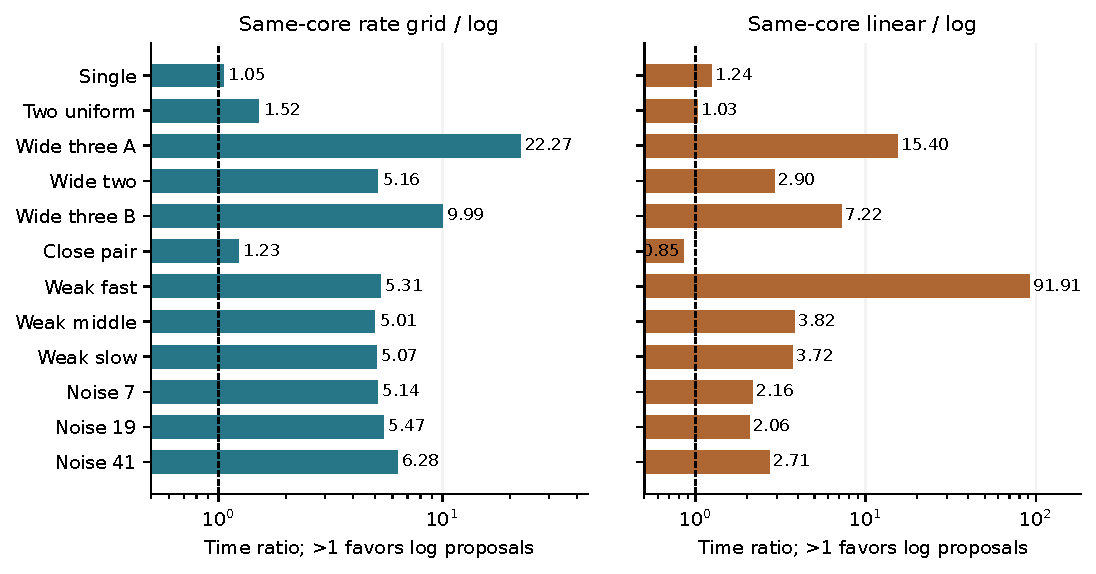
\includegraphics[width=\textwidth]{figures/matched_controls.pdf}
\caption{Ratios of seven-run median times for matched compiled routes.
Values above one favor logarithmic-time proposals. All 256-point routes pass
the fixture count/accuracy criteria. The shared single-mode shortcut contributes
no evidence for wavelets. The wide A and wide two fixtures were pilots.}
\label{fig:matched}
\end{figure}

On wide three B, the log route takes 1.23 ms, versus 8.88 ms for linear
coordinates and 12.29 ms for rate-grid proposals: factors of 7.22 and 9.99.
On the close pair, linear coordinates take 6.80 ms versus 7.96 ms for log
coordinates. The weak-fast case gives the largest coordinate ratio, 91.91,
but it is one clean, development-exposed fixture. The single-mode shortcut
is shared by all native routes. These results support a workload-dependent
proposal-cost benefit, rather than a universal speed ranking.

\subsection{Recovery, noise, and separation}
The reused 480-mixture protocol has 600 observations, one to four components,
amplitudes log-uniform on 0.2--2, and equal numbers of clean and Gaussian-noisy
signals with noise standard deviation 0.001. Logarithmic grids span
0.001--1000, with rates 0.02--60 and adjacent ratios at least three. Uniform
grids span 0.01--20, with rates 0.2--6 and ratios at least two.
Seed 20261107 informed the final count fixes; seed 20261029 was repeatedly
reused. Seed 20261119 was selected before those fixes and was not used to tune
them. The combined result is therefore descriptive validation and regression
evidence. The final method is held fixed for the expanded study.

The new sweep contains 960 noisy signals: two components with amplitudes
1 and 0.5, rates 0.5 and 0.5 times a ratio of 1.1, 1.25, 1.4, 2, 3, or 10;
noise standard deviations 0.0001, 0.001, 0.01, or 0.05; uniform or logarithmic
grids with 600 points on 0.01--20. Each cell has twenty independent realizations
from seed 2026102101. Protocol and source hashes were frozen before inspecting
outcomes; no core tuning followed this evaluation.

\begin{table}[htbp]
\centering\small
\caption{Count recovery on the reused 480-mixture set and the new 960-observation sweep. Legacy rate errors are the conditional 95th percentile of the largest per-mixture relative error, in percent, for noisy correctly counted cases. The final column also requires the stated reconstruction and rate-error targets. Pencil denominators include only uniform grids.}\label{tab:research-counts}
\begin{tabular}{@{}lrrrr@{}}
\toprule
Method & Legacy counts & Legacy 95th (\%) & Sweep counts & Sweep pass \\
\midrule
Log wavelets & 480/480 & 5.40 & 708/960 & 573/960 \\
Linear wavelets & 477/480 & 5.42 & 708/960 & 580/960 \\
Native grid & 480/480 & 5.40 & 737/960 & 568/960 \\
Variable projection & 479/480 & 5.40 & 737/960 & 613/960 \\
Pencil + refinement & 235/240 & 7.29 & 323/480 & 280/480 \\
\bottomrule
\end{tabular}
\end{table}


Clean accuracy targets require the true count, normalized maximum reconstruction
error at most $10^{-8}$, and largest relative rate error at most $10^{-5}$.
Noisy targets require the true count, clean-signal RMSE no greater than the
noise standard deviation, and largest relative rate error at most 10\%.
Rate errors pair sorted true and fitted rates and are undefined for incorrect
counts. Joint-pass fractions retain all eligible observations in their denominator.

The log route recovers 480/480 legacy counts; variable projection recovers
479/480. In the new sweep both coordinate detectors recover 708/960 counts,
while variable projection recovers 737/960. Requiring both count and accuracy
reduces these totals to 573/960 and 613/960 for log wavelets and variable
projection, respectively. Among correctly counted log-wavelet fits, the new
95th-percentile rate error is 31.85\%; the largest is approximately 6,989\%.
A correct count can therefore describe the wrong individual rates. These
extreme errors remain in the records and are failures of the joint target.

\begin{figure}[htbp]
\centering
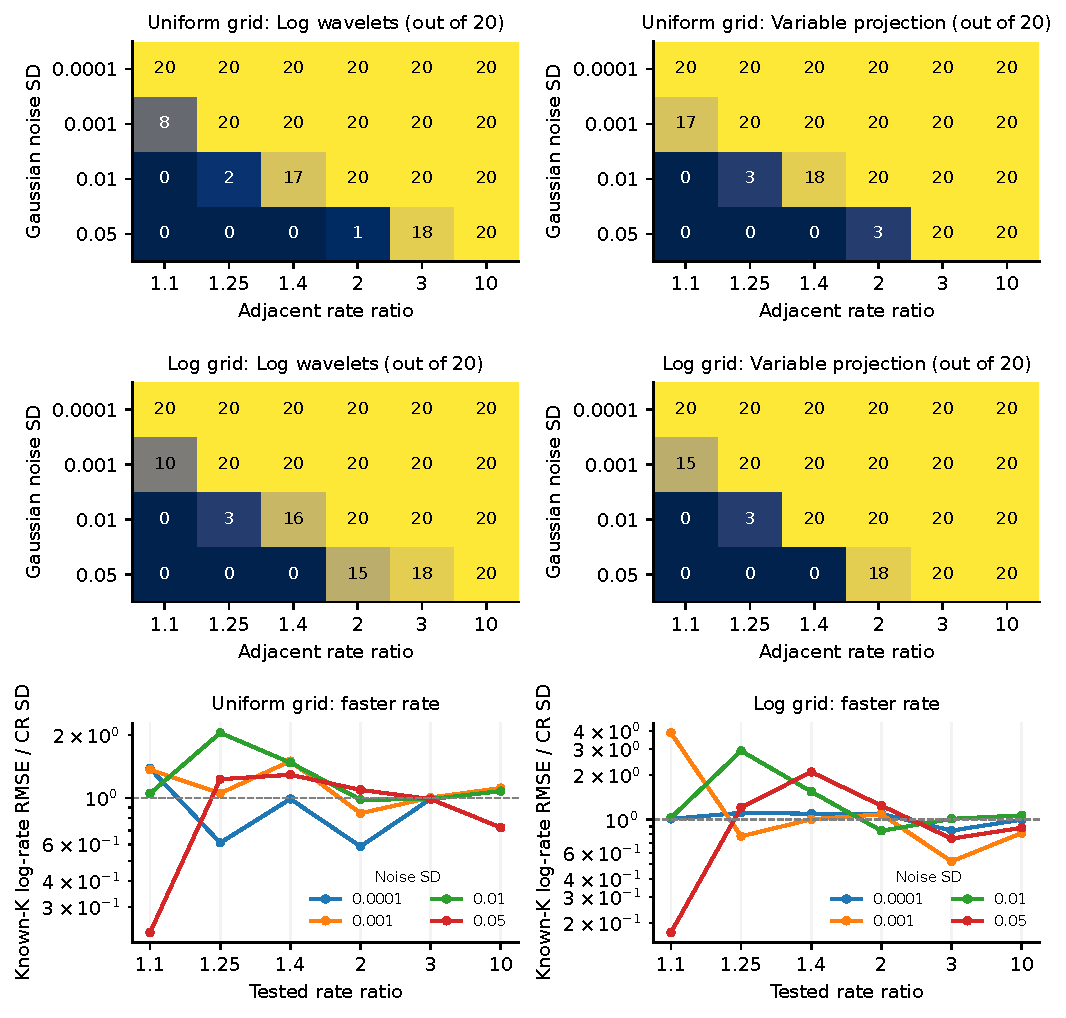
\includegraphics[width=\textwidth]{figures/noise_sweep.pdf}
\caption{New sweep: correct-count totals out of twenty realizations per cell
(top four panels). Bottom panels compare true-count variable-projection
log-rate RMSE with the local Cramer--Rao standard deviation for the faster rate.
All twenty fits enter each RMSE. Ratios below one can reflect finite-sample
variation and estimator bias; they do not invalidate the bound.}
\label{fig:sweep}
\end{figure}

\subsection{Local information and configuration sensitivity}
For known count and independent Gaussian noise, the full amplitude/log-rate
Jacobian $J$ gives the local information bound \cite{kay}
\begin{equation}
\mathcal I=J^{\mathsf T}J/\sigma^2,
\qquad \operatorname{Cov}(\hat\theta)\succeq\mathcal I^{-1}.
\label{eq:crb}
\end{equation}
Amplitudes are nuisance parameters. The covariance inequality requires the
usual regularity and unbiasedness conditions; it is not a bound on one fitted
error or on biased, count-selecting estimates. SVD rank checks avoid reporting
zero uncertainty in unidentifiable directions. Figure~\ref{fig:sweep} also
reports unconditioned true-count RMSE; numerical records retain empirical bias.

For the legacy worst-rate-error case, true-count variable projection reproduces
the same 21.07\% error as the log route. The corresponding rate's local log-rate
standard deviation is 0.197, consistent with weak identifiability. This agreement
does not prove global optimality or statistical efficiency. Public-default retry
preserves 480/480 legacy counts. Increasing the linear detector to 1024 points
instead gives 376/480, showing that more interpolation points alone do not
ensure better selection.

\subsection{Measured fluorescence tails}
An open TCSPC archive provides unquenched prompt and delayed fluorescence curves
for 4CzIPN \cite{experiment}. Original CSVs, IRF columns, units, CC BY 4.0
attribution, and hashes are retained. A predeclared tail gate starts after both
five bins beyond the decay peak and the last IRF bin above 1\% of its maximum.
The median of the last 10\% of decay bins estimates background. Four-bin
averaging reduces data size; negative background-corrected values are retained.

\begin{figure}[htbp]
\centering
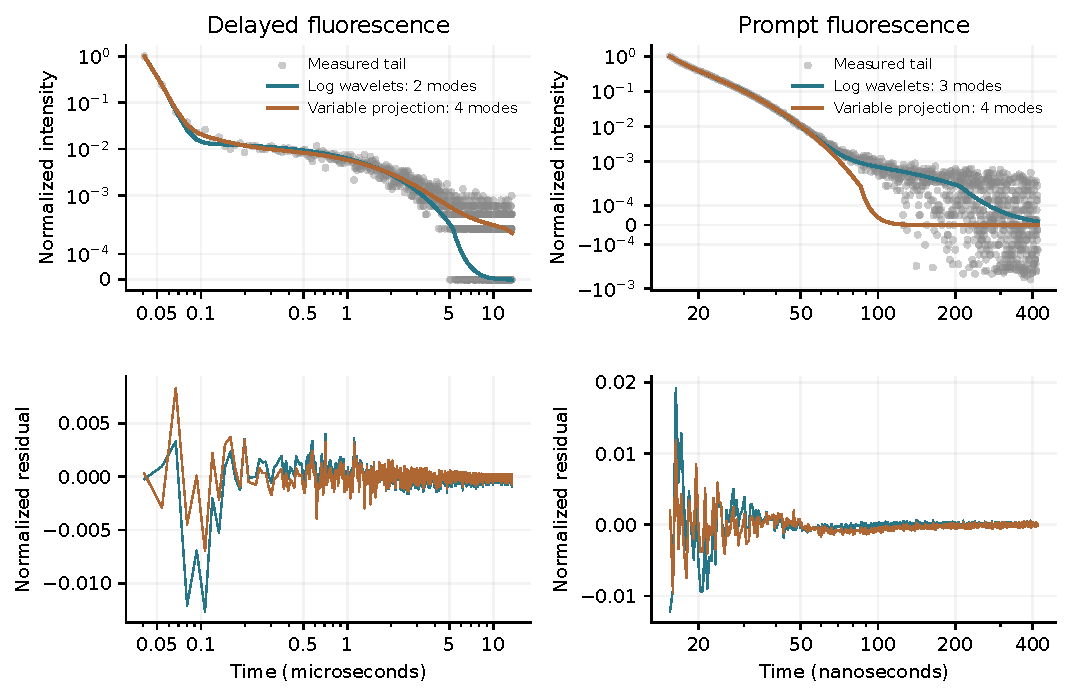
\includegraphics[width=\textwidth]{figures/experimental_tails.pdf}
\caption{Measured fluorescence tails and descriptive fits after fixed gating,
background subtraction, and four-bin averaging. Residuals share the normalization
of each curve. The log-wavelet and variable-projection reconstructions differ
in their tails and selected counts. No independent component truth is available.}
\label{fig:experiment}
\end{figure}

\begin{table}[htbp]
\centering\small
\caption{Descriptive unweighted fits to measured fluorescence tails. RMSE is in original intensity units after four-bin averaging. The additional gate is a predeclared sensitivity check. Component truth is unavailable; lower residuals do not establish physically correct components.}\label{tab:experimental}
\begin{tabular}{@{}lrrrr@{}}
\toprule
Tail / gate & Log K & Log RMSE & VarPro K & VarPro RMSE \\
\midrule
Delayed, +0 bins & 2 & 1.099 & 4 & 0.835 \\
Delayed, +5 bins & 4 & 0.719 & 4 & 0.719 \\
Prompt, +0 bins & 3 & 12.123 & 4 & 9.065 \\
Prompt, +5 bins & 3 & 7.595 & 4 & 6.875 \\
\bottomrule
\end{tabular}
\end{table}


Figure~\ref{fig:experiment} and Table~\ref{tab:experimental} show lower residuals
for variable projection. Delaying the gate by five additional bins changes
the log route's delayed-fluorescence count from two to four. This application
therefore demonstrates preprocessing sensitivity, not verified molecular
components. Photon noise is heteroscedastic; the IRF is gated rather than
convolved. These unweighted fits require a more specific observation model
before physical lifetime interpretation.

\section{Impact and limitations}
LaplaceX provides automatic initial proposals and an inspectable component
representation for small mixtures, reducing repeated fitting work in suitable
multiscale problems. The native controls give direct evidence for proposal-cost
gains; specialist comparisons and the noise sweep establish their limits.
Neither the matched linear control nor the variable-projection implementation
represents every possible method in its class. A continuous-spectrum comparison,
additional machines, sample-count scaling, signed-mixture stress tests, and
noise models matched to specific instruments remain outside this evaluation.

The numerical release is recent. Its 149 original tests and successful public
CI establish a tested software snapshot, not long-term research adoption.
Eight additional tests check evaluation machinery and the version 1.1.0
amplitude-weight alias; all 157 pass. Serious earlier numerical errors and their
corrections remain in the historical audit. Weeks inversion still fails some
singular or discontinuous examples, and oscillatory inputs can require more
terms. Version 1.0.0 should not be read as a uniform numerical guarantee.

\section{Conclusions}
Logarithmic-time wavelet proposals reduce search cost for several separated-rate
workloads under matched native controls. The harder sweep and experimental
tails show that this gain does not ensure superior count recovery or precise
individual rates. LaplaceX is useful as an automatic fitting workflow whose
outputs remain subject to identifiability, model checks, and application-specific
validation.

\clearpage
\section*{Software and data availability}
The MIT-licensed numerical core is release 1.0.0 at the version-pinned repository
in the metadata table. The accompanying research directory supplies frozen
protocols, external controls, baseline implementations, all outcomes, and
source/binary hashes. The Python alias, additional tests, and research files accompany version
1.1.0; the numerical algorithms used here are unchanged.
The measured CSVs are redistributed with the original authors' CC BY 4.0
attribution. Reproduction requires the released core checkout plus the
accompanying research files; the research files are not claimed to exist in
the release's original pinned commit.

\bibliographystyle{elsarticle-num}
\bibliography{references}
\end{document}
